\documentclass[]{article}

\usepackage{caption}
\usepackage{graphicx, subfig}
\usepackage{listings}
\usepackage[namelimits]{amsmath} 
\usepackage{fontspec}
\usepackage{amsmath}
\usepackage{amssymb}                      
\usepackage{mathrsfs}  
\usepackage{amsfonts}   
\setmainfont[Mapping=tex-text]{KaiTi}
\usepackage{fullpage}
\usepackage{amsthm}
\usepackage{fancyhdr}
\usepackage{algorithm}
\usepackage{algorithmic}
\usepackage{bm}
\usepackage{ctex}
\usepackage{txfonts}

\usepackage[usenames,dvipsnames]{xcolor}

%opening
\title{统计机器学习 课后作业5}
\author{陈劭涵 17300180049}



\newcommand{\tm}{\fontspec{Times New Roman}}


\begin{document}
	
\maketitle


\section{问题1(1)}
\begin{flushleft}
解:
\end{flushleft}
设极大似然中的参数为:$P(Y=c_k)$, $P(X^{(j)}=a_{jl}|Y=c_k)$\\\\
其中$a_{jl}$是$X$的第$j$个分量可能取的第$l$个值,取值域为$S_j$\\\\
$I(Y=c_k)$在$Y=c_k$满足时取$1$,否则取$0$\\\\
对于先验概率:\\\\
$P(Y=c_k)=P(Y=c_k)^{I(Y=c_k)}(1-P(Y=c_k))^{1-I(Y=c_k)}$\\\\
极大似然估计:\\\\
$l(P(Y=c_k))=arg\ max_{P(Y=c_k)} \ log(\prod_{i=1}^{N} P(Y_i=c_k)^{I(Y_i=c_k)}(1-P(Y_i=c_k))^{1-I(Y_i=c_k)})$\\\\
$=arg\ max_{P(Y=c_k)} \sum_{i=1}^{N} log(P(Y_i=c_k)^{I(Y_i=c_k)}(1-P(Y_i=c_k))^{1-I(Y_i=c_k)})$\\\\
$=arg\ max_{P(Y=c_k)} (\sum_{Y_i=c_k}logP(Y_i=c_k)+\sum_{Y_i\neq c_k}logP(1-P(Y_i=c_k)))$\\\\
$=arg\ max_{P(Y=c_k)} (\sum_{i=1}^{N}I(Y_i=c_k)logP(Y_i=c_k)+\sum_{i=1}^{N}I(Y_i\neq c_k)log(1-P(Y_i=c_k))$\\\\
上式关于$P(Y=c_k)$求导\\\\
$\frac{dl(P(Y=c_k))}{dP(Y=c_k)}=\frac{d(\sum_{i=1}^{N}I(Y=c_k)logP(Y=c_k)+\sum_{i=1}^{N}I(Y\neq c_k)log(1-P(Y=c_k)))}{dP(Y=c_k)}=\frac{\sum_{i=1}^{N}I(Y_i=c_k)}{P(Y_i=c_k)}-\frac{\sum_{i=1}^{N}I(Y\neq c_k)}{1-P(Y_i=c_k)}=0$\\\\
根据上式,又$\because \sum_{i=1}^{N}I(Y_i=c_k)+\sum_{i=1}^{N}I(Y_i\neq c_k)=N$\\\\
$\therefore$根据极大似然估计$P(Y=c_k)=\frac{\sum_{i=1}^{N}I(Y=c_k)}{N}$\\\\
对于条件概率:\\\\
$P(X^{(j)}=a_{jl}|Y=c_k)=\frac{P(X^{(j)}=a_{jl},Y=c_k)}{P(Y=c_k)}$\\\\
为方便表示,将$P(X^{(j)}=a_{jl},Y=c_k)$简写为$P$,并将指示函数写为$I$\\\\
当$X^{(j)}=a_{jl}$且$Y=c_k$的时候,$I$取$1$,否则取$0$\\\\
极大似然估计:\\\\
$l(P)=arg\ max_{P}\sum_{X}log(P^I(1-P)^{1-I})$\\\\
$=arg\ max_{P}(\sum_{i=1}^{N}IlogP+\sum_{i=1}^{N}(1-I)log(1-P))$\\\\
同理,对上式关于$P$求导\\\\
$\frac{dl(P)}{dP}=\frac{\sum_{i=1}^{N}I}{P}-\frac{\sum_{i=1}^{N}(1-I)}{1-P}=0$\\\\
根据上式,又$\because \sum_{i=1}^{N}I(Y_i=c_k)+\sum_{i=1}^{N}I(Y_i\neq c_k)=N$\\\\
$\therefore P(X^{(j)}=a_{jl},Y=c_k)=\frac{\sum_iI(x_i^{(j)}=a_{jl},y_i=c_k)}{N}$\\\\
$\therefore$根据极大似然估计$P(X^{(j)}=a_{jl}|Y=c_k)=\frac{P(X^{(j)}=a_{jl},Y=c_k)}{P(Y=c_k)}=[\frac{\sum_iI(x_i^{(j)}=a_{jl},y_i=c_k)}{N}]/ [\frac{\sum_{i=1}^{N}I(Y=c_k)}{N}]=\frac{\sum_iI(x_i^{(j)}=a_{jl},y_i=c_k)}{\sum_iI(y_i=c_k)}$\\\\
\section{问题1(2)}
\begin{flushleft}
	解:
\end{flushleft}
极大似然估计:\\\\
计算先验概率:\\\\
$P(Y=1)=\frac{\sum_{i=1}^{N}I(Y=1)}{N}=\frac{10}{15}=\frac{2}{3}$\\\\
$P(Y=-1)=\frac{\sum_{i=1}^{N}I(Y=-1)}{N}=\frac{5}{15}=\frac{1}{3}$\\\\
计算条件概率:\\\\
$P(X^{(1)}=2|Y=1)=\frac{\sum_{i=1}^{N}I(X^{(1)}=2,Y=1)}{\sum_{i=1}^{N}I(Y=1)}=\frac{2}{10}=\frac{1}{5}$\\\\
$P(X^{(2)}=M|Y=1)=\frac{\sum_{i=1}^{N}I(X^{(2)}=M,Y=1)}{\sum_{i=1}^{N}I(Y=1)}=\frac{4}{10}=\frac{2}{5}$\\\\
$P(X^{(1)}=2|Y=-1)=\frac{\sum_{i=1}^{N}I(X^{(1)}=2,Y=-1)}{\sum_{i=1}^{N}I(Y=-1)}=\frac{3}{5}$\\\\
$P(X^{(2)}=M|Y=-1)=\frac{\sum_{i=1}^{N}I(X^{(2)}=M,Y=-1)}{\sum_{i=1}^{N}I(Y=-1)}=\frac{2}{5}$\\\\
计算后验概率:\\\\
$P(Y=1|X^{(1)}=2,X^{(2)}=M)=\frac{2}{3}\times(\frac{1}{5}\times\frac{2}{5})=\frac{4}{75}$\\\\
$P(Y=-1|X^{(1)}=2,X^{(2)}=M)=\frac{1}{3}\times(\frac{3}{5}\times\frac{2}{5})=\frac{2}{25}\geq P(Y=1|X^{(1)}=2,X^{(2)}=M)$\\\\
$\therefore$在极大似然估计下,给定输入的类标记是-1\\\\
贝叶斯估计:\\\\
计算先验概率:\\\\
$P(Y=1)=\frac{\sum_{i=1}^{N}I(Y=1)+\lambda}{N+2\times \lambda}=\frac{11}{17}$\\\\
$P(Y=0)=\frac{\sum_{i=1}^{N}I(Y=-1)+\lambda}{N+2\times \lambda}=\frac{6}{17}$\\\\
计算条件概率:\\\\
$P(X^{(1)}=2|Y=1)=\frac{\sum_{i=1}^{N}I(X^{(1)}=2,Y=1)+\lambda}{\sum_{i=1}^{N}I(Y=1)+2\times\lambda}=\frac{3}{13}$\\\\
$P(X^{(2)}=M|Y=1)=\frac{\sum_{i=1}^{N}I(X^{(2)}=M,Y=1)+\lambda}{\sum_{i=1}^{N}I(Y=1)+2\times\lambda}=\frac{5}{13}$\\\\
$P(X^{(1)}=2|Y=-1)=\frac{\sum_{i=1}^{N}I(X^{(1)}=2,Y=-1)+\lambda}{\sum_{i=1}^{N}I(Y=-1)+2\times\lambda}=\frac{4}{8}=\frac{1}{2}$\\\\
$P(X^{(2)}=M|Y=-1)=\frac{\sum_{i=1}^{N}I(X^{(2)}=M,Y=-1)+\lambda}{\sum_{i=1}^{N}I(Y=-1)+2\times\lambda}=\frac{3}{8}$\\\\
计算后验概率:\\\\
$P(Y=1|X^{(1)}=2,X^{(2)}=M)=\frac{11}{17}\times(\frac{3}{13}\times\frac{5}{13})=\frac{165}{2873}$\\\\
$P(Y=-1|X^{(1)}=2,X^{(2)}=M)=\frac{6}{17}\times(\frac{1}{2}\times\frac{3}{8})=\frac{72}{1088}\geq P(Y=1|X^{(1)}=2,X^{(2)}=M)$\\\\
$\therefore$在贝叶斯估计下,给定输入的类标记是-1
\section{问题3}
\begin{flushleft}
	解:
\end{flushleft}
(1):
\begin{lstlisting}[language=R]
train=read.csv("D:/大数据学院文件资料/2020秋课程/机器学习/assignment/homework5/
市长电话分析/train_set.csv")
val=read.csv("D:/大数据学院文件资料/2020秋课程/机器学习/assignment/homework5/
市长电话分析/test_set.csv")

num=table(train$单位名称)
num=sort(num,decreasing = TRUE)
num
colors=colorRampPalette(c("coral2", "gold"))(length(num))
bar=barplot(num,col=colors,main="政府单位投诉量降序柱状图",
xlab="政府单位名称",ylab="投诉量",ylim=c(0,600))
\end{lstlisting}
降序统计结果:
\begin{lstlisting}[language=R]
> num

市水务集团   市供热公司 市运输管理局   市燃气集团   市公交集团   市房地集团   市供电公司 
557          332          330          285          207           96           93 
\end{lstlisting}
降序柱状图为:\\\\
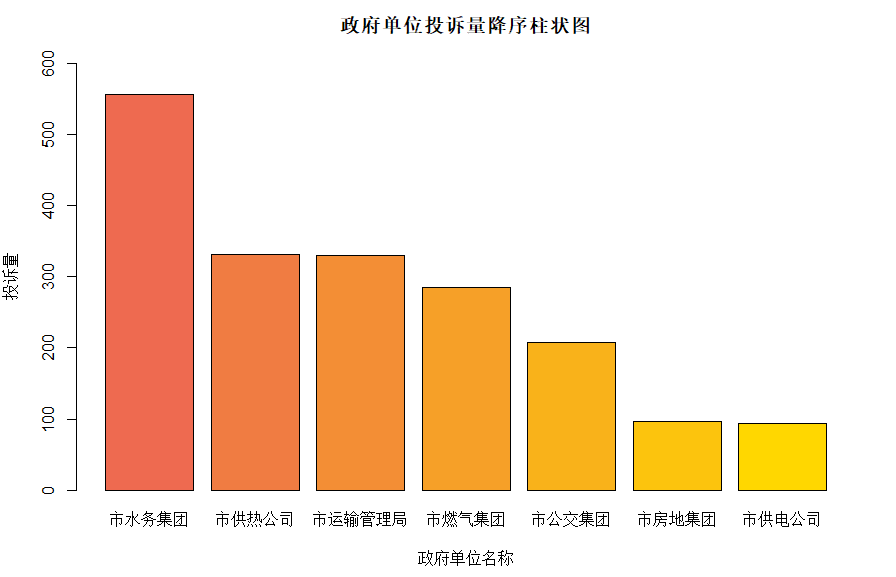
\includegraphics[width=1.\textwidth]{D:/大数据学院文件资料/2020秋课程/机器学习/homework/hw5/1.png}\\\\
解读:\\
1、在训练集中共有7个政府单位被投诉。可以看到不同政府单位街道的市民投诉量差别较大。投诉量分布于100至550次范围内;\\
2、被投诉最多的是市水务集团,达到550多次,并且大大高于其他单位的投诉量,说明该市的水务集团的服务质量不好,接到较多投诉;被投诉最少的是市供电公司和市房地集团,说明这两个单位的服务质量相对较高;其他单位接到的投诉量在他们之间,说明他们的服务质量相对好于水务集团,但差于房地集团和供电公司。\\\\
(2):
\begin{lstlisting}[language=R]
words=apply(train[-1],1,sum)
hist=hist(words,col=c("yellow","coral","firebrick1",rainbow(30)),
main="每条投诉的用词数量直方图",
xlab="投诉用词数",ylab="分布数量",breaks=30,ylim=c(0,500))
\end{lstlisting}
直方图如下:\\\\
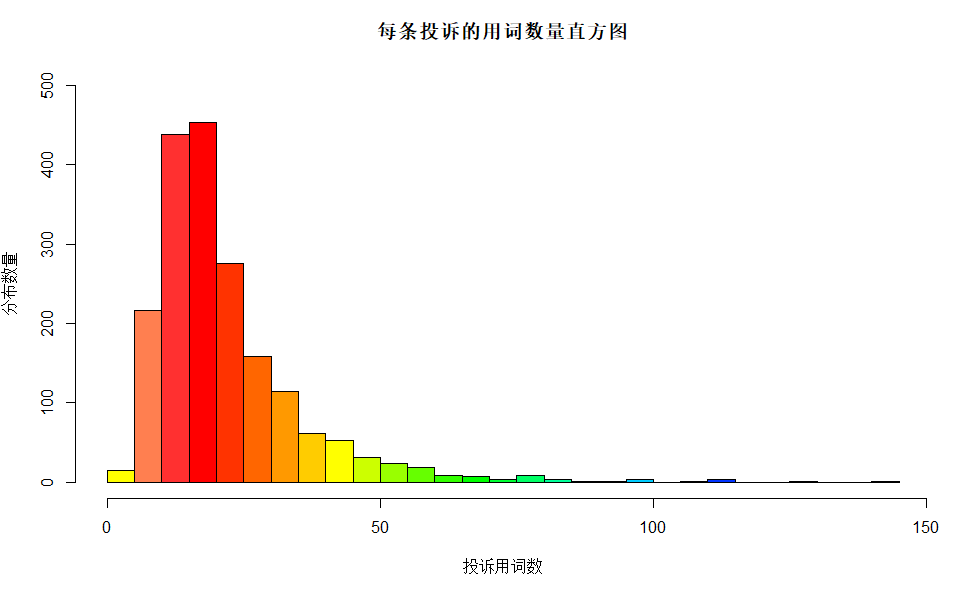
\includegraphics[width=1.\textwidth]{D:/大数据学院文件资料/2020秋课程/机器学习/homework/hw5/2.png}\\\\
从直方图中我们可以看到:\\
1、绝大部分的投诉用词都在50词以下,其中最高的投诉用词达到144个词;\\
2、非常大一部分的投诉都在10至30词之间,少数的用词超过50词,极少数会超过100词,整体分布是右偏的;\\\\
(3):\\\\
\begin{lstlisting}[language=R]
boxplot(words~单位名称,data=train,col=rainbow(7),border=c("dimgray","dimgrey"),
main='每条投诉信息词汇量~单位名称的箱线图',names=单位名称,
xlab="单位名称",ylab="每条投诉信息词汇量",plot=T)
\end{lstlisting}
箱线图如下:\\\\
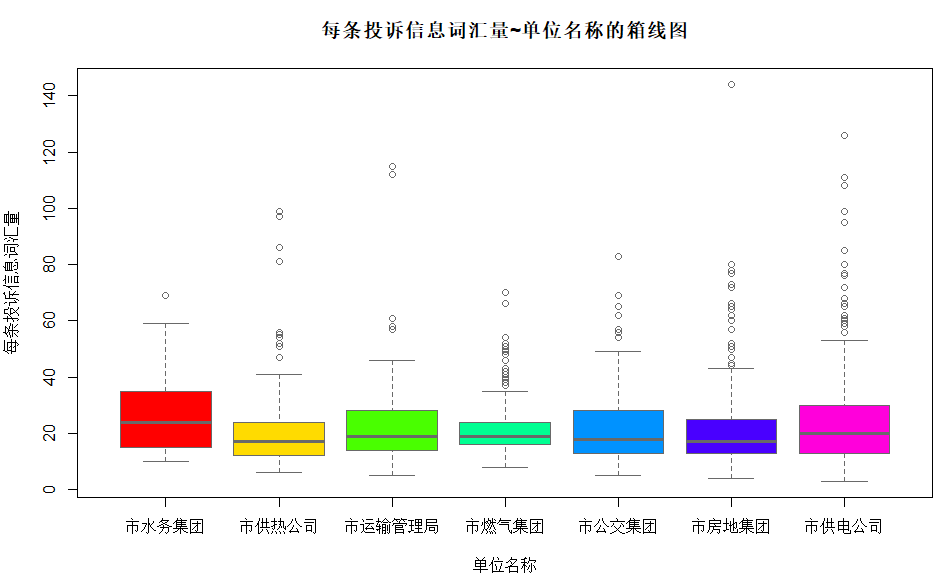
\includegraphics[width=1.\textwidth]{D:/大数据学院文件资料/2020秋课程/机器学习/homework/hw5/3.png}\\\\
为了可视化方便,我们对纵坐标取对数再做一次箱线图:
\begin{lstlisting}[language=R]
boxplot(log(words)~单位名称,data=train,col=rainbow(7),border=c("dimgray","dimgrey"),
main='log(每条投诉信息词汇量)~单位名称的箱线图',names=单位名称,
xlab="单位名称",ylab="log(每条投诉信息词汇量)",plot=T)
\end{lstlisting}
对数箱线图如下:\\\\
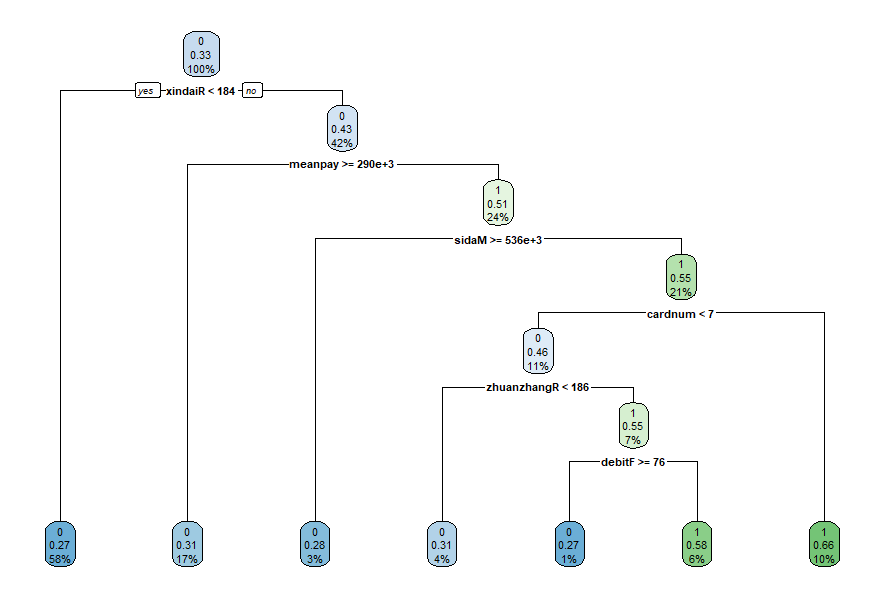
\includegraphics[width=1.\textwidth]{D:/大数据学院文件资料/2020秋课程/机器学习/homework/hw5/4.png}\\\\
从如上箱线图中我们可以看到:\\
1、针对各政府部门的每条投诉信息所使用的词汇量分布各不相同;从分布特性上看,市水务集团和市供电公司以及市公交集团的每条投诉信息词汇量的分布最不均匀,分布范围最广;市燃气集团和市供电公司的词汇量分布范围相对较紧;\\
2、除了市水务集团,其他政府部门的投诉信息词汇量均有较多的高值离群值,这表明有一些市民使用了较大篇幅的投诉来表明自己遇到的问题;\\
3、市水务集团遇到的每条投诉信息用词数相对较多,房地集团和供热公司遇到的每条投诉信息用次数相对较少,说明可能需要水务集团出面解决的问题需要更多的词汇才能准确描述,而市民描述其他单位的投诉问题所需要的词汇数相对较少;与之前的投诉量降序柱状图相联系,我们发现市水务集团不仅收到的投诉最多,平均每条投诉所用词的数目也是最多的;\\\\
(4):
\begin{lstlisting}[language=R]
train[,-1]=(train[,-1]>=1) 
val[,-1]=(val[,-1]>=1)
library("e1071")
bayes=naiveBayes(train$单位名称~.,train)
bresult=predict(bayes,val)
sum(val$单位名称==bresult
\end{lstlisting}
预测结果为:
\begin{lstlisting}[language=R]
> sum(val$单位名称==bresult)
[1] 97
\end{lstlisting}
说明在测试集的100个样例中,朴素贝叶斯模型成功预测了其中的97个样例\\\\
接下来我们展示混淆矩阵并画图
\begin{lstlisting}[language=R]
library("graphics")
pred=bresult 
real=val$单位名称
cm=as.matrix(as.data.frame.matrix(table(pred,real)))
cm
breaks.frequency=seq(from=min(cm), to=max(cm), length.out=10)
myColors=colorRampPalette(c("white", "#2874A6"))

draw=function(cm,axis=TRUE,label=TRUE){
	image(1:nrow(cm),1:ncol(cm),cm,breaks=breaks.frequency, 
	col=myColors(length(breaks.frequency)-1),axes=F,cex=2,
	xlab="预测类别",ylab="真实类别")
	if (axis){  
		for (x in 1:nrow(cm)) {
			for (y in 1:ncol(cm))  {
				text(x, y, cm[x,y],cex=2)
			}
		}
	}
	if(label){
		axis(2, 1:ncol(cm), colnames(cm), cex.axis=0.7)
		axis(1, 1:nrow(cm), rownames(cm), cex.axis=0.7)
	}
}
draw(cm)
\end{lstlisting}
混淆矩阵:
\begin{lstlisting}[language=R]
> cm
       市房地集团 市公交集团 市供电公司 市供热公司 市燃气集团 市水务集团 市运输管理局
市房地集团     4          0          0          0          0          0            0
市公交集团     0         15          0          0          0          0            0
市供电公司     0          0          3          0          0          0            0
市供热公司     2          0          0         17          0          0            0
市燃气集团     0          0          0          0         12          0            0
市水务集团     0          0          1          0          0         32            0
市运输管理局   0          0          0          0          0          0           14
\end{lstlisting}
混淆矩阵画图:\\\\
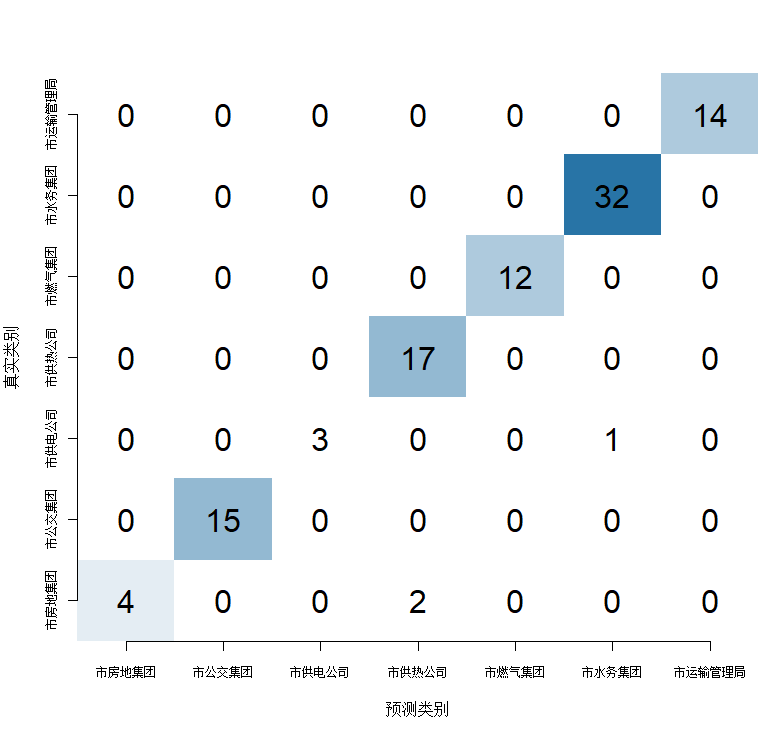
\includegraphics[width=.8\textwidth]{D:/大数据学院文件资料/2020秋课程/机器学习/homework/hw5/5.png}\\\\
\end{document}
